\documentclass[9pt,twocolumn,twoside]{../../styles/osajnl}
\usepackage{fancyvrb} \journal{i524}

\title{Detecting Street Signs in Videos in a Robot Swarm}

\author[1,*]{Rahul Raghatate} 
\author[1]{Snehal Chemburkar}

\affil[1]{School of Informatics and Computing, Bloomington, IN 47408,
  U.S.A.}

\affil[*]{Corresponding authors: rraghata@iu.edu, snehchem@iu.edu}

\dates{S17-IR-P003, \today}

\ociscodes{Street Signs, Video Streams, OpenCV, Spark, Cloud}


\doi{\url{https://github.com/cloudmesh/sp17-i524/raw/master/project/S17-IR-P003/report/report.pdf}}

\begin{abstract}
The aim of this project is to deploy a software package to detect
street signs in a video stream. This will be a scalable
system over Hadoop based cloud ecosystem to incorporate multiple video
feeds and parallel real-time processing of the feeds. A comparative
benchmark will be developed based on the performance of package on
multiple cloud systems.\newline
\end{abstract}

\setboolean{displaycopyright}{true}

\begin{document}

\maketitle

\section{Introduction}
Detecting objects in images has always been keen area of interest in
the field of computer vision. There are many applications developed
based on this simple idea like auto tagging pictures (e.g. Facebook,
Phototime), counting the number of people in a
street(e.g. Placemeter), classifying pictures, detecting vehicles,
etc. On the similar grounds, we are building a software package which
can be deployed easily on cloud infrastructure and establish a
platform to detect different street signs in a video stream. A
benchmark will be developed based on performance of this software on
different cloud systems. The database of street signs will be
restricted to US street signs. The video streams used for this project
are simulated or captured using mobile camera.

The purpose of this project is to deploy a street sign detection algorithm on a cloud infrastructure to enable distributed processing of the images and videos. Detection and classification of street signs is an important feature in the era of autonomous driving vehicles. The market for autonomous driving and advanced driver assisted systems (ADAS) has increased the interest in the field of traffic sign detection techniques. Benchmarks have been created for the traffic sign detections on the German and Belgium Traffic Sign Datasets \cite{paper-trafficsign}. The only publicly available dataset for US traffic signs is the LISA dataset \cite{paper-lisadataset} which very huge. In this project, we have collected data by clicking photos of street signs, grabbing images from google and from the LISA dataset \cite{paper-lisadataset}. 

Image processing is a vast field and due to limited knowledge in this field we restrict ourselves to the basic image processing required to detect objects in street signs. Processing images and videos in real time requires a lot of computing power and this is where the cloud systems come in. We leverage the distributed computing power of Spark on Yarn for faster processing of images and videos. This solution is deployed on two different clouds to benchmark the deployment and processing of the algorithm for different workloads.

\section{Requirement Analysis}
We are using following technologies for complete project development
and deployment:
\begin{itemize}
\item Cloudmesh provides command line interface to connect to different cloud systems.
\item Ansible - Ansible is an automated software deployment tool that only runs on the host machine.
\item Python - Programming language. 
\item Spark - Distributed computing engine.
\item YARN - is the resource manager for Spark.

\item OpenCV \cite{www-opencv} - Image/video analysis for street sign detection using open source computer vision libraries.The OpenCV library provides several features to  manipulate images(apply filters, transformation), detect and recognize objects in images.
\end{itemize}

\section{Methodology}
\begin{enumerate}
\item Data gathering for street signs and video streams
\item Deploy Hadoop clusters on cloud using Cloudmesh
\item Develop Ansible script to install OpenCV on cloud
\item Build a model to detect or track street signs using OpenCV. We
  plan on implementing two programs-
    \begin{itemize}
    \item Read an image and run the Haar cascade classifier to detect
      the signs in the image and
    \item use the video stream and detect signs in real time.
    \end{itemize}
\item To detect street signs, we will be using Haar based cascade
  classifier which detect objects in an image. As detecting signs and
  categorizing them are two different problems and use two different
  approaches. Hence, we will benchmark detection first and will work
  on categorization as future development.
\item Test the performance of software package on 3 different clouds
  or on the same cluster with multiple nodes.
\item Create benchmarks based on the above results

\end{enumerate}

\section{Execution Summary}
This section specifies the week by week timeline for project
completion.

\begin{enumerate}
\item {Mar 6 - Mar 12, 2017: } Create virtual machines on Chameleon
  cloud using Cloudmesh and submit the project proposal.
\item {Mar 13-Mar 19, 2017: } Deployed Hadoop cluster to Chameleon cloud
  using Cloudmesh and develop Ansible playbook to install the required
  software packages to the clusters (OpenCV, Python and dependencies)
\item {Mar 20-Mar 26, 2017: } Collated data for training and test data sets and trained stop sign classifier. Developed Ansible playbook to deploy Hadoop and Spark to the cloud machines.
\item {Mar 27-Apr 02, 2017: } Trained data for stop and yield sign classifiers
  using OpenCV.  Developed Ansible playbook to setup the OpenCV python environment on Spark clusters.
\item {Apr 03-Apr 09, 2017: } Trained data for signal ahead sign
  using OpenCV. Test stop sign classifier on local machine and chameleon cloud.
\item {Apr 10 - Apr 16, 2017: } Tested classifier on Spark and created deployable software package using shell script.
\item {Apr 17-Apr 23, 2017: } Completed project report and developed benchmarks for the project.
\end{enumerate}

\begin{figure*}[h]\centering
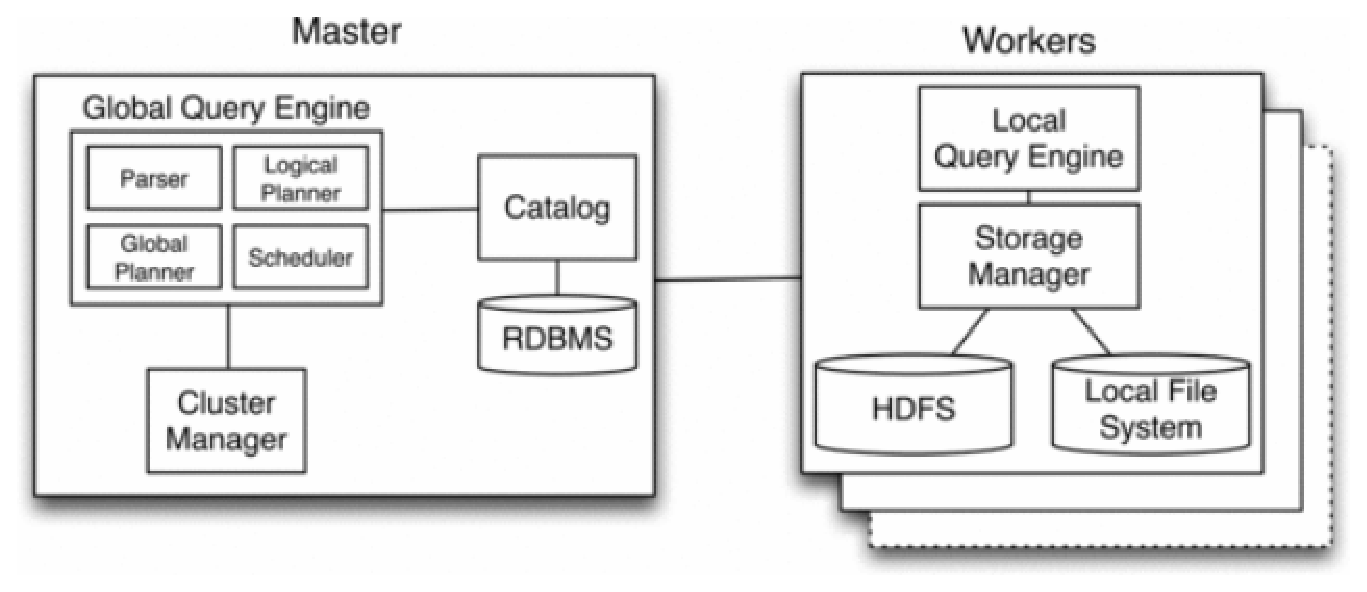
\includegraphics[width=\linewidth]{images/architecture}
\caption{System Architecture}
\label{fig:enter,update & exit}
\end{figure*}

\section{System Architecture}

Figure shows an overview of our system architecture, the host machine being our laptop in this case. Ansible and Cloudmesh client are installed on this host machine. Roles are defined in the Ansible playbook for each of the different steps in the deployment process. We execute the Ansible playbooks to instantiate the cloud machines, deploy Hadoop and Spark on them and then carryout the street detection processing on Spark using Yarn resource manager. When we submit our job to Spark, the driver program initializes the SparkContext object which is responsible for the execution of the job. The data is parallelized and sent to the worker nodes for processing. Yarn acts as the resource manager and provides executors to the worker nodes. The output is saved to the local file system on the master node and transferred to the host machine through a script.

\section{Cloud Infrastructure}
For the purpose of this project, we have been provided with two clouds – Chameleon and Jetstream. 
Chameleon cloud is a National Science Foundation funded experimental testbed that provides large scale cloud services to "members of the US computer Science research community and its international collaborators \cite{www-chameleon}." Jetstream allows researchers to leverage the computational power of cloud while retaining the look and feel of home machines. Jetstream adds cloud based computational power to the national cyberinfrastructure, which was led by the Indiana University Pervasive Technology institute \cite{www-jetstream}.

\section{Cloudmesh}
Cloudmesh provides an easy interface to multiple clouds such as Chameleon and Jetstream through the command line.  
\begin{verbatim} 
cm cluster define –count 3 
\end{verbatim} 
defines a set of cluster machine instances. 
Cloudmesh client can be installed via pip. It is a lightweight utility that enables users to connect to different clouds from their laptops or computers. Users can customize Cloudmesh client to suite their needs of cyberinfrastructure. It provides simple command line scripts to deploy Hadoop with Spark addon to either of the clouds mentioned in section 5. 

\section{Ansible Automation}
Ansible is an easy to use, opensource automation tool that is used to automate the deployment of our project on the cloud infrastructure. Ansible is an agentless tool, that is, it does not require ansible to be deployed on the remote machines. It runs only on the host machine to deploy the required processes to the remote machines through SSH authentication.
Using Ansible, we can create modules for each step of the deployment process and define the roles individually. An inventory file is used to define the machines in groups as required. A sample inventory file looks like: 
\begin{verbatim} 
[master] 
192.128.0.1 
[workernode] 
192.168.0.2 
192.168.0.3 
\end{verbatim}

\section{OpenCV Image Processing}

OpenCV provides a range of computer vision algorithms to detect objects in images. One of the simplest method for object detection is based on color. The results of Color based detection method are largely affected by the lighting conditions and one require the user to calibrate multiple times before they might get a better result in the real world. Hence this technique is not very popular when detecting objects in the real world
Haar features is a sophisticated technique that uses the features specific to the object in question. It been seen that working with RGB pixel values in every single pixel in the image results in computationally expensive and slow feature calculation. “A Haar-like feature considers neighboring rectangular regions at a specific location in a detection window, sums up the pixel intensities in each region and calculates the difference between these sums. This difference is then used to categorize subsections of an image \cite{paper-objectdetection}.” OpenCV provides a Haar feature based cascade classifier that can be used for object detection, as proposed by in \cite{paper-ROD}. 

\subsection{Data Collection}

The publicly available data set for U.S street signs is the LISA traffic dataset \cite{paper-lisadataset}. This dataset contains images for 47 different traffic signs. But since the data set itself is approximately 7GB, we extracted 50 images from the dataset for the purpose of testing. For our training set, we captured images of street signs and put together a few positive images for the street signs. The positive images were cropped to only contain the street sign and resized to 50x50.

\subsection{Train a Haar feature-based Cascade Classifier}

Based on tutorials provided in \cite{www-coding-robin}, [2] and [3], we carried out multiple experiments to train a classifier to detect street signs. Since each sign needed to trained separately, we picked stop, yield, and signal ahead signs to start with. To train a classifier, we firstly required gathering at least a few positive and many negative images. The positive images are images of the object alone cropped to a size of 24x24 or 50x50 whereas the negative images should not contain the object in consideration here. In case we have a single positive image or a few positive images, OpenCV provides a utility called opencv\_createsamples to generate the training and test datasets in *.vec format that is supported by the opencv\_traincascade utility. The samples generated from the opencv\_createsamples can be passed to the opencv\_traincascade utility to get a trained classifier.   
Multiple experiments were carried out by differing the sample sizes (the width by height of the positive images) and varying the number of positive and negative images. As the dataset and width by height increases the computational time increases. Below are the trainings that were carried out for stop sign:

\begin{verbatim}
opencv_traincascade -data classifier -vec samples.vec 
-bg negatives.txt  -numStages 20 -minHitRate 0.999 
-maxFalseAlarmRate 0.5 -numPos 120 -numNeg 200 -w 50
-h 50 -mode ALL -precalcValBufSize 1024
-precalcIdxBufSize 1024
\end{verbatim}
\begin{verbatim}
opencv_traincascade -data classifier -vec samples.vec 
-bg negatives.txt  -numStages 20 -minHitRate 0.999 
-maxFalseAlarmRate 0.5 -numPos 200   -numNeg 350 
-w 50 -h 50 -mode ALL -precalcValBufSize 1024 
-precalcIdxBufSize 1024
\end{verbatim}
\begin{verbatim}
opencv_traincascade -data classifier -vec samples.vec
-bg negatives.txt  -numStages 20 -minHitRate 0.999 
-maxFalseAlarmRate 0.5 -numPos 600   -numNeg 100 -w 50 
-h 50 -mode ALL -precalcValBufSize 1024 
-precalcIdxBufSize 1024
\end{verbatim}

When we increased the number of positive samples to 600 for the 50x50 image size, the training ran for 3.5 days. The resulting classifier was unable to detect the stop signs in the test data. After a couple more experiments and another week invested in training the classifier to no good results, we found success with a pre-trained classifier for stop signs available at \cite{github-stopsigns}. The results of this classifier are shown in \ref{fig:detect}.

\begin{figure}[htbp]
\centering
\fbox{\includegraphics[width=\linewidth]{images/detection.jpg}}
\caption{Stop Sign Detection}
\label{fig:detect}
\end{figure}

After successful testing of Stop sign classifier, we proceeded to train the classifiers for Yield sign and Signal Ahead sign. We trained 3 classifiers each for both these signs while increasing the number of positive images from 600, 900, 1200. Even after increasing the number of positive images up to 1200 the resulting classifiers were not efficient enough to detect the signs in images.
As each training had resulted in a loss of approximately 3.5 days,  we realized that this could not be covered as part of this project and restricted ourselves to the stop sign detection. 
\subsubsection{Learnings}
\begin{itemize}
\item From the many experiments we carried out, we learned that there is no fixed number of samples that will yield a decent result. 
\item Future work can be done on training the U.S traffic signs, since there are no classifiers available for them . With the growing market for autonomous vehicles and assisted driving technology, having trained classifiers for the traffic signs might prove to helpful.
\end{itemize}

\section{Programming Environment}
Programming for the analysis module of the project was done in Python. OpenCV provides a library that can be used for running computer vision algorithms in Python. We leverage the Pyspark  API provided by Spark to execute this module in Spark distributed environment. Ansible deployment scripts are written in YAML format which is similar to giving commands in plain English. Finally, the benchmarking for the project is done using shell script to calculate the processing times for each of the steps in the deployment method.

\section{Benchmark}
Benchmarks will be created based on the performance of the software in
different cloud environments. \ref{fig:jmedium} shows the graph for time taken for the complete deployment on Jetstream when the number of images parsed are 4. It can been seen from the graph that as the number of nodes is increased the processing time is reduced. \ref{fig:cmedium4} and \ref{fig:cmedium50} reflect the performance of Chameleon cloud for 4 and 50 input images respectively. \ref{fig:jmedium4} and \ref{fig:jmedium50} reflect the performance of Jetstream for 4 and 50 input images respectively. There are a few outliers which can be attributed to the network delays and user input delays. Overall these benchmarks clearly reflect that as the number of nodes increases the processing time decreases. Due to limited resources on Jetstream, the processing times for 3 node clusters could not be obtained. 

\begin{figure}[htbp]
\centering
\fbox{\includegraphics[width=\linewidth]{images/jetstream4.JPG}}
\caption{Total time on Jetstream with 4 Input Images}
\label{fig:jmedium}
\end{figure}


\begin{figure}[htbp]
\centering
\fbox{\includegraphics[width=\linewidth]{images/Cmedium4.jpg}}
\caption{Performance on Chameleon Cloud with 4 Input Images}
\label{fig:cmedium4}
\end{figure}

\begin{figure}[htbp]
\centering
\fbox{\includegraphics[width=\linewidth]{images/Cmedium50.jpg}}
\caption{Performance on Chameleon Cloud with 50 Input Images}
\label{fig:cmedium50}
\end{figure}

\begin{figure}[htbp]
\centering
\fbox{\includegraphics[width=\linewidth]{images/jmedium4.jpg}}
\caption{Performance on Jetstream with 4 Input Images}
\label{fig:jmedium4}
\end{figure}

\begin{figure}[htbp]
\centering
\fbox{\includegraphics[width=\linewidth]{images/jmedium50.jpg}}
\caption{Performance on Jetstream with 50 Input Images}
\label{fig:jmedium50}
\end{figure}

\section{Use Cases}
\begin{enumerate}
\item Street Sign Detection for autonomous vehicles.
\item Analysis of traffic signs in Google Street View to estimate all
  signs ahead hence, useful in ambulance , fire brigade services,
  simplest path finder etc.
\end{enumerate}


\section{Future Work}
This work can be expanded to detect and classify all the U.S traffic signs. Benchmarks can be developed for them similar to the German and Belgium Traffic Sign Detection and Classification benchmarks. 


\section*{Acknowledgements}
This project is undertaken as part of the I524: Big Data and Open
Source Software Projects coursework at Indiana University. We would
like to thank our Prof. Gregor von Laszewski, Prof. Gregory Fox and
the Associate Instructors for their help and support. Results presented in this paper were obtained using the Chameleon testbed supported by the National Science Foundation.

% Bibliography
\bibliography{references}

\section*{Author Biographies}
\begingroup \setlength\intextsep{0pt}
\begin{minipage}[t][3.2cm][t]{1.0\columnwidth}
% Adjust height [3.2cm] as required for separation of bio photos.
  \begin{wrapfigure}{L}{0.25\columnwidth}
    \includegraphics[width=0.25\columnwidth]{images/rahul_thumbnail.jpg}
  \end{wrapfigure}
  \noindent
  {\bfseries Rahul Raghatate} will receive his Masters (Data Science)
  in 2018 from The Indiana Univeristy Bloomington. His research
  interests include Big Data and Machine Learning.
\end{minipage}
\begin{minipage}[t][3.2cm][t]{1.0\columnwidth} % Adjust height [3.2cm] as required for separation of bio photos.
  \begin{wrapfigure}{L}{0.25\columnwidth}
    \includegraphics[width=0.25\columnwidth]{images/alice_smith.eps}
  \end{wrapfigure}
  \noindent
  {\bfseries Snehal Chemburkar} will receive her Masters (Data
  Science) in 2018 from Indiana University Bloomington. Her research
  interests include Big Data and Machine Learning.
\end{minipage}
\endgroup

\appendix

\end{document}
